\section{Modello di sviluppo}
Abbiamo adottato un modello di sviluppo che suddivide il tempo in macroperiodi e questi ultimi in microperiodi. I macroperiodi sono scanditi dalle revisioni di progetto. I microperiodi durano una settimana.

\subsection{Inizio del progetto}
All'inizio del progetto abbiamo individuato tutte le attività che dovranno essere eseguite per portarlo a termine.
Abbiamo suddiviso le attività nei 4 macroperiodi.
\subsection{Macroperiodo}
All'inizio di ogni macroperiodo il responsabile assegna a ogni macroattività di quel periodo delle ore.
Alla fine del macroperiodo il responsabile redige un consuntivo delle ore utilizzate realmente, e in base a questo un preventivo a finire dei macroperiodi successivi. Questo PaF potrà essere utilizzato, eventualmente con qualche modifica, come pianificazione all'inizio del macroperiodo successivo.
\subsection{Microperiodo}
All'inizio di ogni microperiodo il responsabile:
\begin{enumerate}
	\item sceglie le attività da cominciare o proseguire;
	\item definisce le ore necessarie per svolgere ogni attività, prendendo come riferimento non vincolante la distribuzione oraria eseguita all'inizio del macroperiodo. Questo riferimento non è totalmente vincolante in quanto potrebbe essere necessario svolgere un'attività imprevista (di cui la pianificazione di macroperiodo non può ovviamente tenerne conto) oppure un'attività potrebbe richiedere più tempo di quanto definito durante la pianificazione di macroperiodo;
	\item assegna le attività ai membri di DPCM 2077, garantendo la rotazione dei ruoli e un egual carico orario individuale.
\end{enumerate}  

\indent Alla fine del microperiodo si esegue un consuntivo della settimana e si verifica quali attività sono state completate. Se emergono criticità il responsabile adotterà i necessari provvedimenti per evitare il ripresentarsi di problemi simili. Nel periodo successivo il responsabile utilizzerà queste informazione per pianificare in modo migliore.

La struttura del microperiodo e del macroperiodo è rappresentata nella seguente immagine.
\begin{figure}[H]
	\centering
	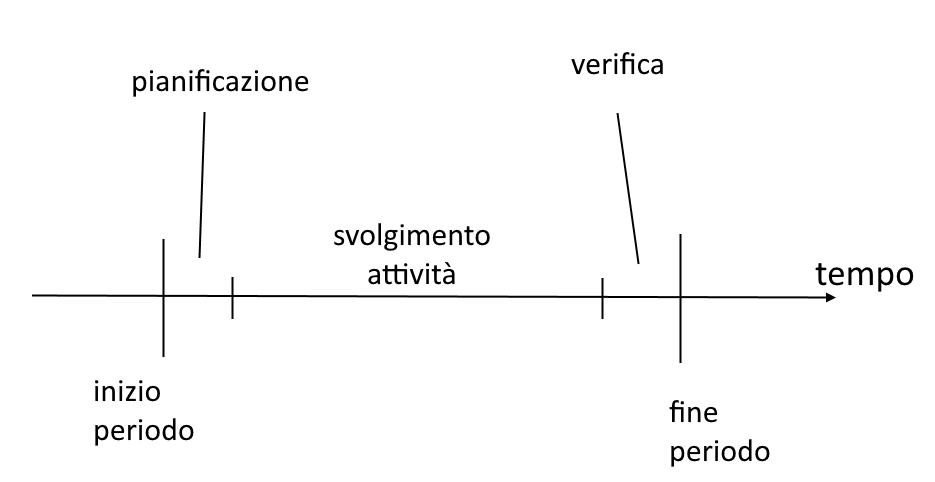
\includegraphics[width=0.7\linewidth]{res/images/schema_periodo.png}
	\caption*{\textbf{Figura 1}: Schema del periodo}
	\label{fig:linea_tempo_periodo}
\end{figure}

\subsection{Monitoraggio}
Gli strumenti di monitoraggio sono raccolti in una cartella su Google Drive accessibile a tutti i componenti del gruppo e sono i seguenti:
\begin{enumerate}
	\item Pianificazione di revisione: tabella rappresentante la suddivisione delle ore all'interno del macroperiodo tra le varie attività e i vari ruoli.
	\item Consuntivo di revisione: tabella rappresentante le ore effettivamente svolte da ogni ruolo per le diverse attività all'interno del macroperiodo.
	\item Pianificazione settimanale: tabella rappresentante la suddivisione delle ore all'interno del microperiodo tra le varie attività, i vari ruoli e le varie persone.
	\item Consuntivo settimanale: tabella rappresentante le ore effettivamente svolte da ogni ruolo per le diverse attività all'interno del microperiodo. La somma dei consuntivi settimanali fornisce il consuntivo di revisione.
	\item Grafici di scostamento settimanale: rappresentano per ogni settimana lo scostamento orario rispetto a quanto pianificato, suddiviso per ruolo e totale.
	\item Istogramma dell'esperienza per ruolo: mostra l'esperienza avuta da ogni componente per ogni ruolo. Viene usato dal responsabile per suddividere i ruoli nelle prossime attività.
	\item Grafico a torta del progresso dell'attività: mostra la percentuale di attività completate rispetto a quelle previste per il macroperiodo.
	\item Istogrammi del confronto orario e di costo: rappresentano il consuntivo orario e di costo per il macroperiodo presente e lo mettono a confronto con la pianificazione di macroperiodo.
\end{enumerate}

\noindent Gli strumenti di monitoraggio dell'attività sono visibili a tutti i componenti del gruppo e ognuno può utilizzarli. In questo modo l'amministratore ha un cruscotto di monitoraggio aggiornato alla fine di ogni settimana che gli dice:
\begin{itemize}
	\item qual è la previsione delle ore che spenderemo (strumenti 1 e 3);
	\item quanto siamo in ritardo o anticipo rispetto alla pianificazione (strumenti 2, 4, 5 e 8);
	\item come le ore sono state distribuite tra i componenti del gruppo (strumento 6);
	\item quante cose sono state fatte e quante ancora da fare (strumento 7).
\end{itemize}


